\section{Aufbau und Durchführung}
\label{sec:Durchführung}
Die Wärmepumpe besteht aus zwei thermisch isolierten Eimer, die mit Wasser
gefüllt die Wärmereservoire darstellen. In jedem Eimer ist eine Kupferschlange durch
die $\ce{Cl2F2C}$, das Transportgas Dichlordifluormethan, fließt.
Das Wasser wird während der Messung umgerührt. Die Temperaturen innerhalb der
Reservoire werden mit digitalen Thermometern bestimmt, die Drücke mit Zeiger-Manometern.
Die Leistung des Kompressors wird mit einem Wattmeter gemessen.

\begin{figure}
      \centering
      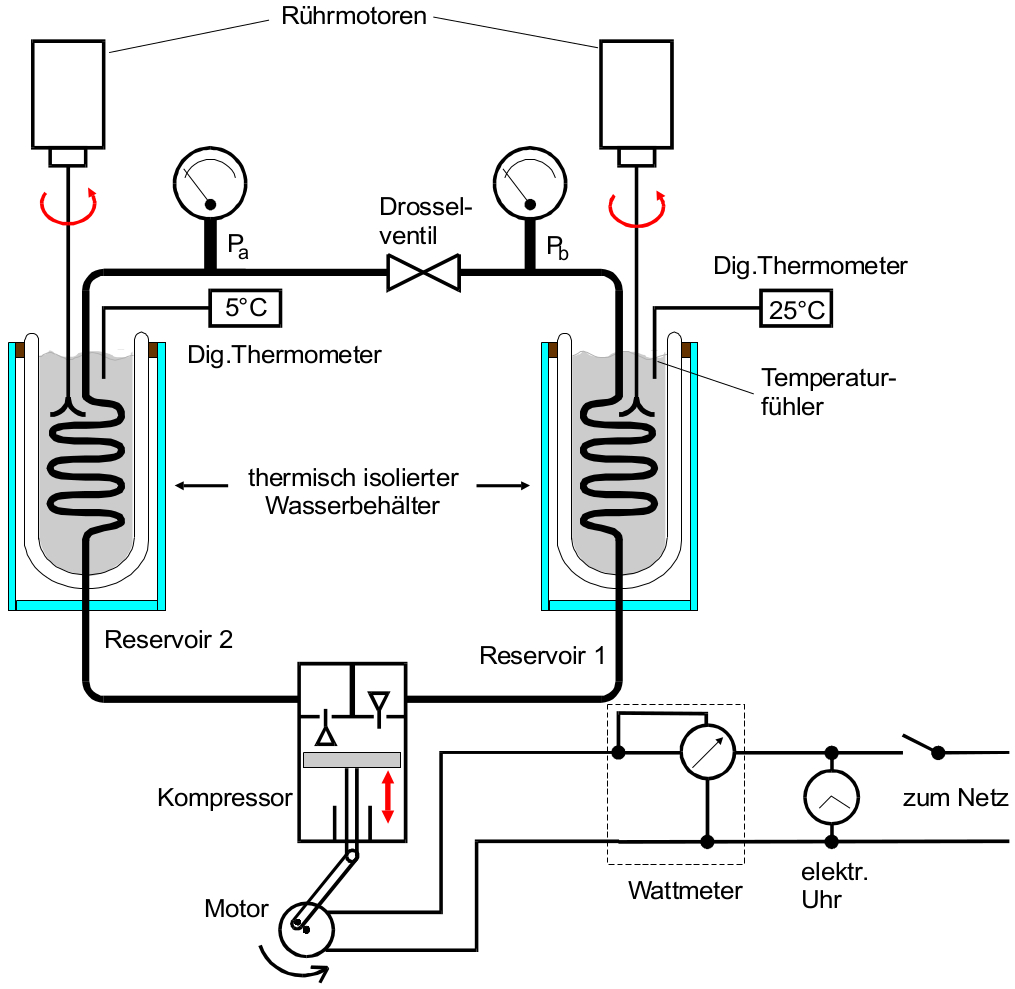
\includegraphics[height=10cm]{content/pumpe.jpg}
      \caption{Schema einer Wärmepumpe aus \cite{Anleitung}.}
      \label{fig:pumpe}
\end{figure}
Die Reservoire sind mit je $\SI{3}{\litre}$ Wasser befüllt.

Gemessen werden die beiden Temperaturen $T_1, T_2$, die beiden Dücke
$p_\text{a}, p_\text{b}$ und die Leistungsaufnahme des Kompressors jede Minute.
Die Messung endet wenn die Temperatur des warmen Reservoirs $T_1 = \SI{50}{\celsius}$
ist.
\begin{table}
      \centering
      \caption{Literaturwerte von Dichlorfluormethan aus \cite{Anleitung}.}
      \label{tab:cl2f2c}
      \sisetup{table-format=1.2}
      \begin{tabular}{S S}
            \toprule
            {$ρ_0\:[\si{\gram\per\litre}]$} & {$\symup{κ}$} \\
            \midrule
            5.51 & 1.14 \\
            \bottomrule
      \end{tabular}
\end{table}

$ρ_0$ für $T = \SI{0}{\celsius},\;p = \SI{1}{\bar}.$
